\documentclass[12pt, a4paper]{book}
\usepackage{amsmath}
\usepackage{geometry}
\usepackage{graphicx}
\usepackage{xurl}
\geometry{paper=a4paper, top=3cm, bottom=3cm, left=2.6cm, right=2.6cm, headheight=14pt,footskip=1.4cm, headsep=10pt}
 
\begin{document}
 
\begin{center}
{\Huge \textbf{Modelling Transit Light Curve through \texttt{Juliet}}}\\
\vspace*{1cm}
{\Huge \textbf{ TOI 1011 }}
\end{center}
 
\vspace*{0.6cm}
 
\begin{center}
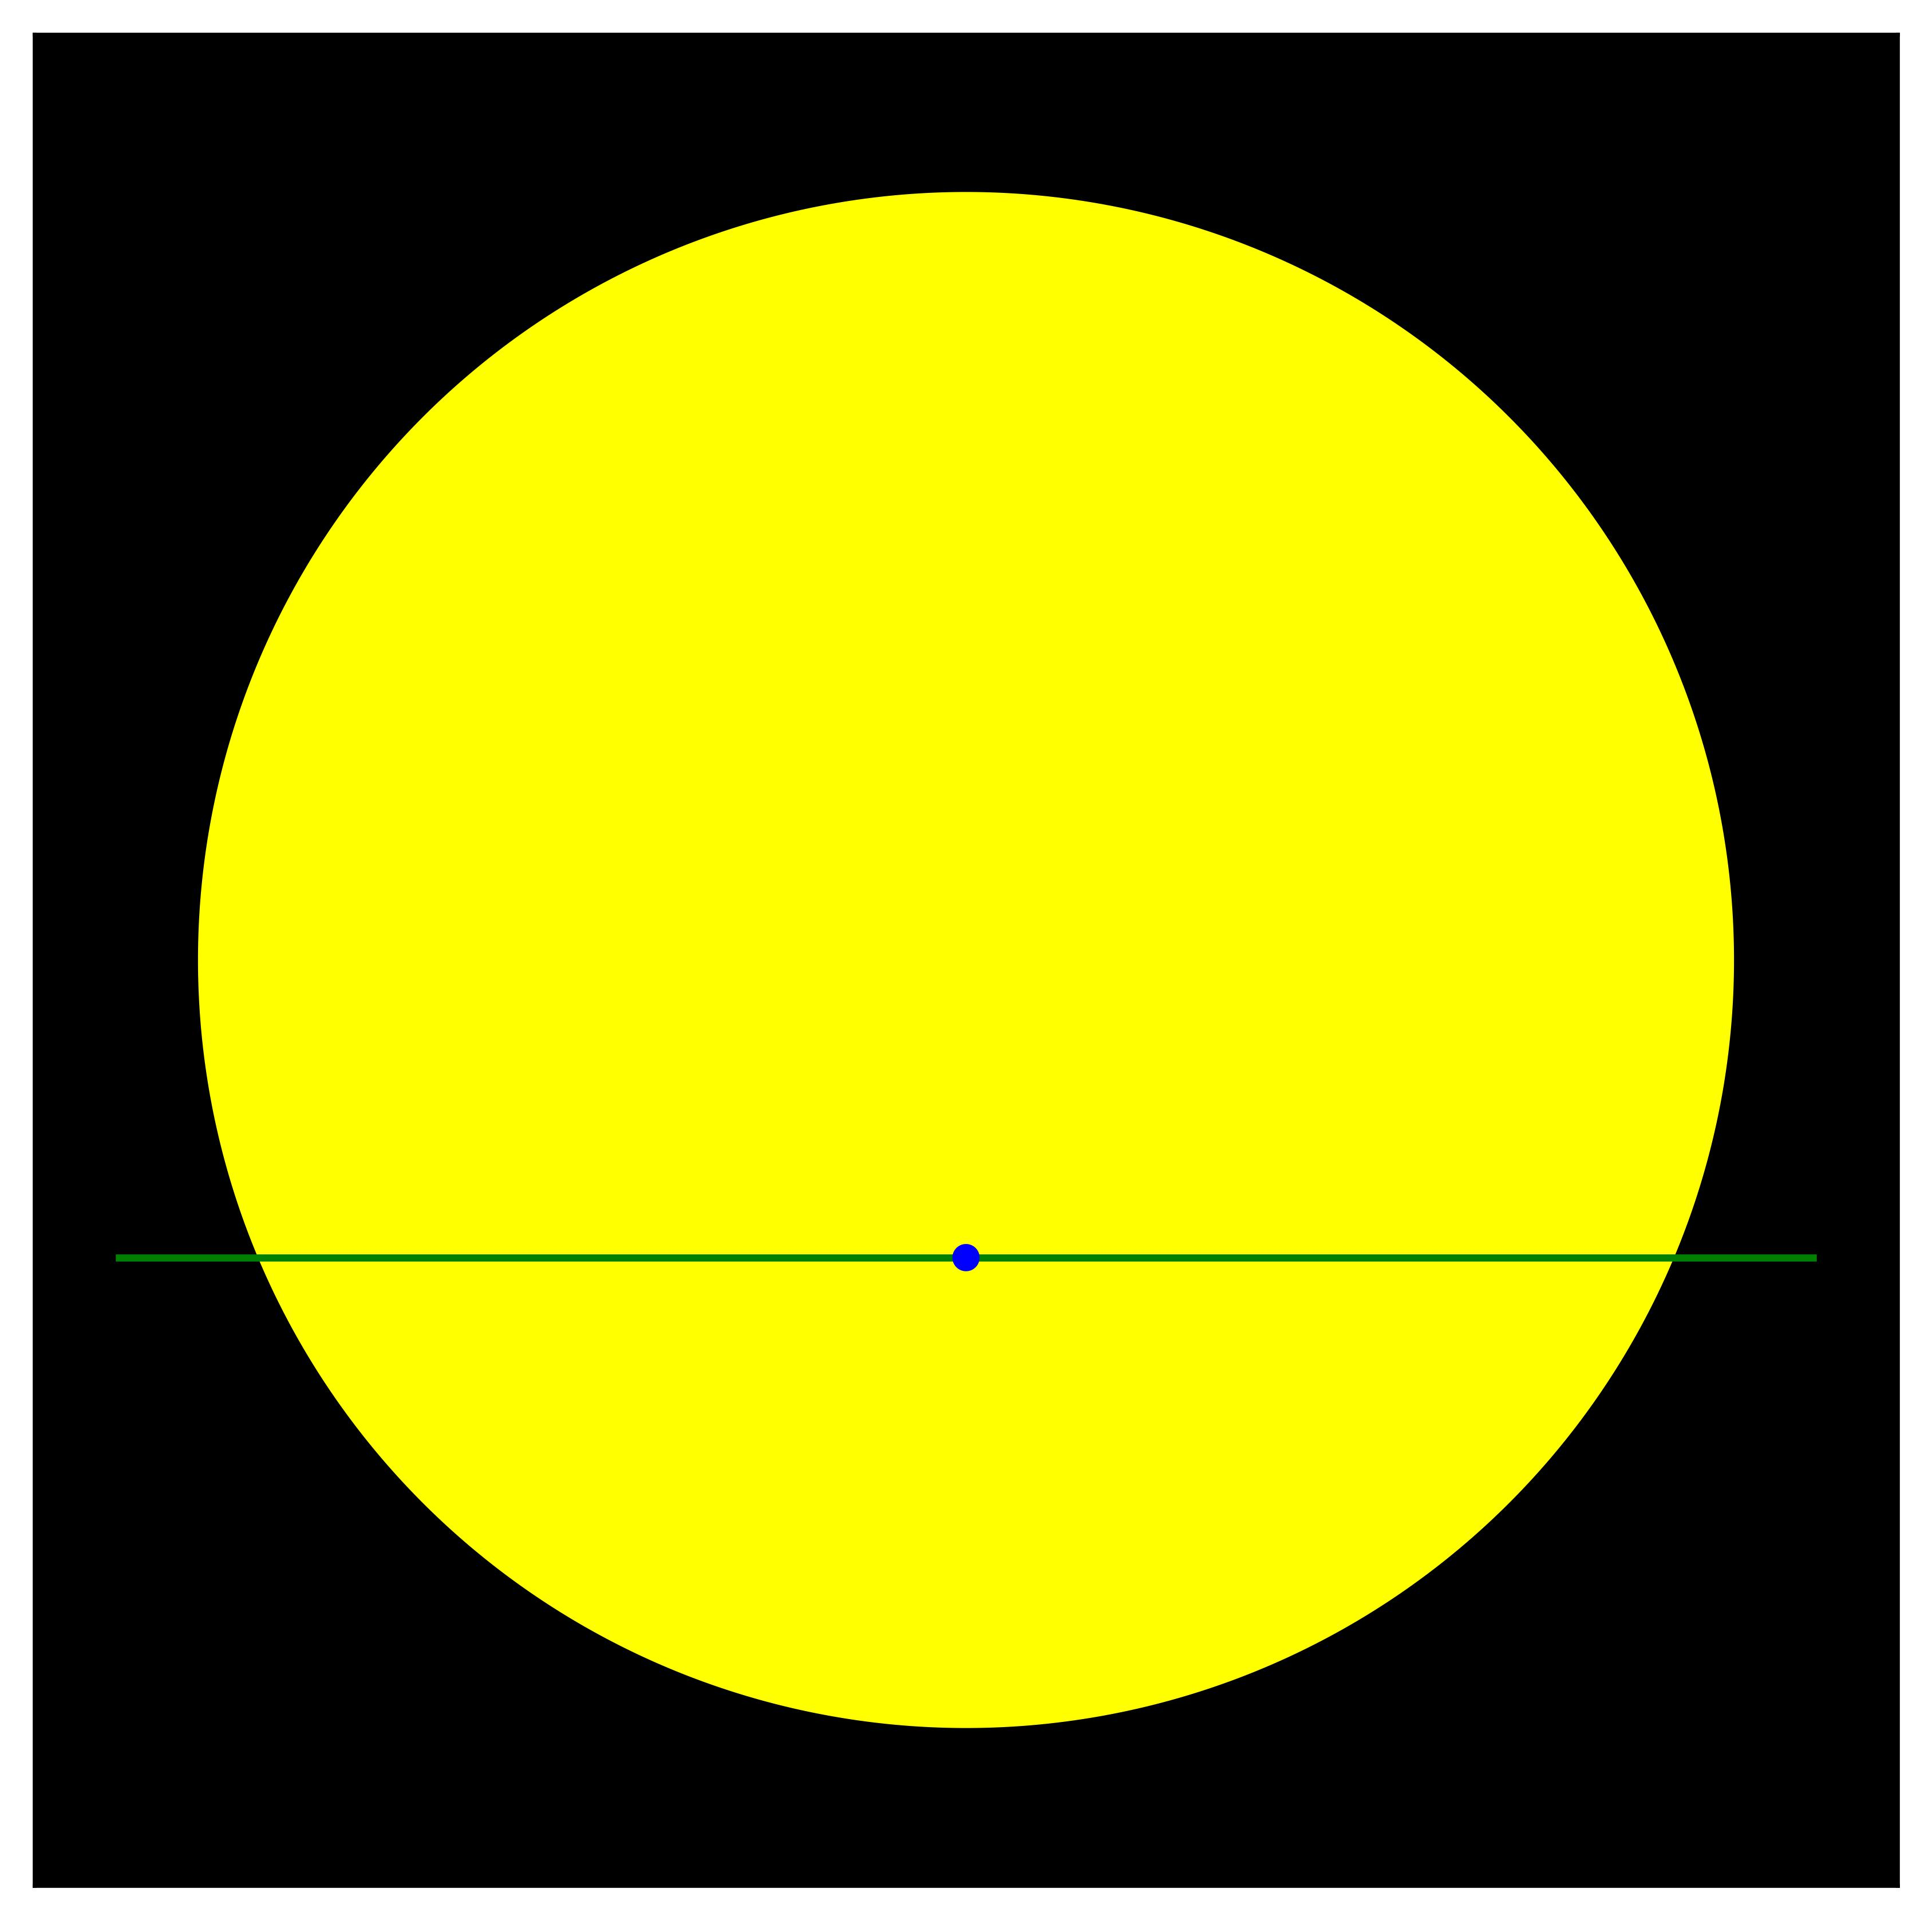
\includegraphics[scale=0.5]{TOI_1011_Visuals}
\end{center}
 
\vspace*{0.6cm}
 
\begin{center}
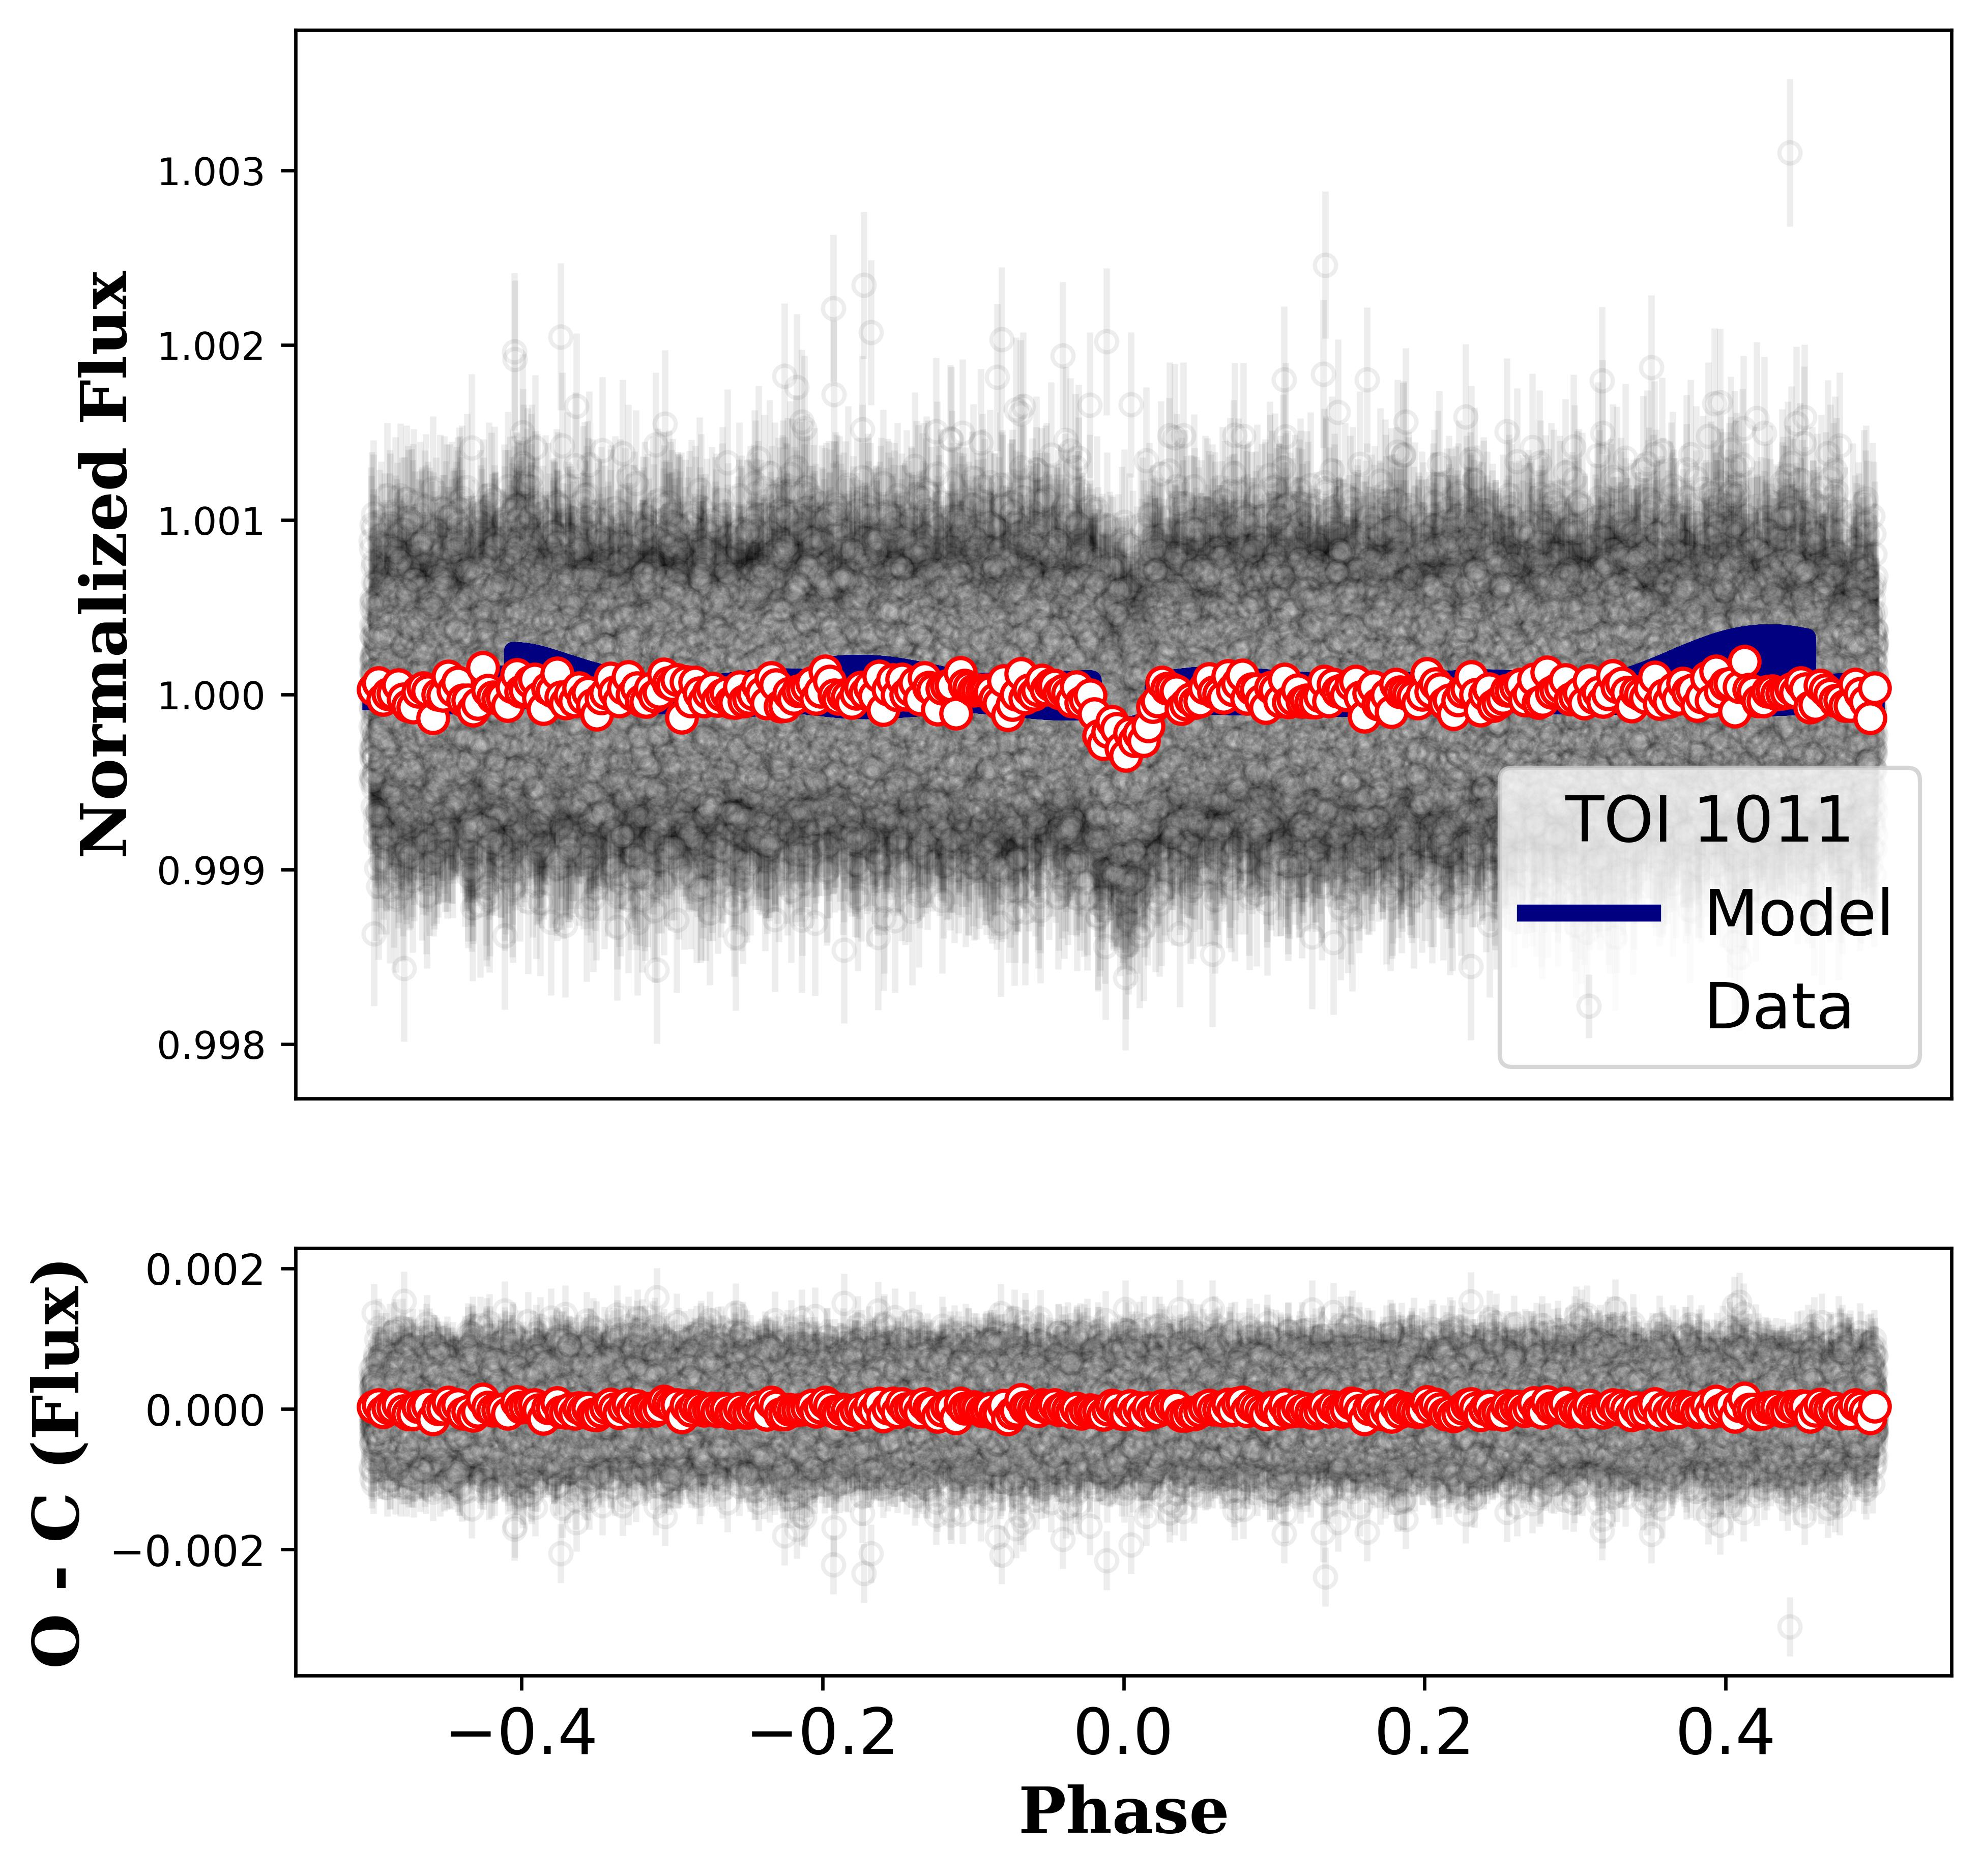
\includegraphics[scale=0.6]{TOI_1011_Transit}
\end{center}
 
\newpage
\begin{center}
{\large \textbf{Stellar Parameters}}
\end{center}
\begin{itemize}
\item Magnitude (V) :  8.2388 $\pm$ 0.006
\item Mass of the Star ($M_*$) :  0.94 $\pm$ 0.119244 $M_\odot$
\item Radius of the Star ($R_*$) :  0.941335 $\pm$ 0.0546131 $R_\odot$
\item Temperature (T) :  5413.68 $\pm$ 132.798 K
\item Luminosity (L) :  0.6857309 $\pm$ 0.0160353 $L_\odot$
\end{itemize}
\vspace*{0.6cm}
\begin{center}
{\large \textbf{Median values and 68\% confidence interval from \texttt{Juliet}}}
\end{center}
 
\begin{center}
\begin{tabular}{c c c}
\hline
\hline
Parameters & Description (Unit) & Values \\
\hline
 & & \\
P & Period (days) & 2.470495 $^{+ 0.000005 } _{- 0.000005 }$ \\
 & & \\
$R_P$ & Radius ($R_J$) & 0.137483 $^{+ 0.000000 } _{- 0.000000 }$ \\
 & & \\
$R_P$ & Radius ($R_E$) & 1.508644 $^{+ 0.000000 } _{- 0.000000 }$ \\
 & & \\
$T_C$ & Epoch Time (BJD) & 2459231.128038 $^{+ 0.001242 } _{- 0.001413 }$ \\
 & & \\
$T_d$ & Transit Duration (days) & 0.098171 $^{+ 0.042908 } _{- 0.030458 }$ \\
 & & \\
$a$ & Semi-major Axis (AU) & 0.032745 $^{+ 0.000000 } _{- 0.000000 }$ \\
 & & \\
$i$ & Inclination (Degree) & 87.032058 $^{+ 2.152472 } _{- 4.364433 }$ \\
 & & \\
$e$ & Eccentricity & 0 (Fixed) \\
 & & \\
$\omega$ & Argument of Periastron (Degree) & 90 (Fixed) \\
 & & \\
$T_{eqq}$ & Equilibrium Temperature (K) & 1400.300528 $^{+ 0.000000 } _{- 0.000000 }$ \\
 & & \\
$S$ & Insolation ($S_E$) & 639.529355 $^{+ 14.954912 } _{- 14.954912 }$ \\
 & & \\
$R_P/R_S$ & Radius of planet in stellar radii & 0.014663 $^{+ 0.001236 } _{- 0.000725 }$ \\
 & & \\
$a/R_S$ & Semi-major axis in stellar radii & 7.473304 $^{+ 0.619632 } _{- 1.821364 }$ \\
 & & \\
$\delta$ & Transit Depth (Fraction) & 0.000215 $^{+ 0.168644 } _{- 0.098930 }$ \\
 & & \\
$b$ & Impact Parameter & 0.388707 $^{+ 0.340393 } _{- 0.273165 }$ \\
 & & \\
$u_1$ & Limb Darkening Parameter & 0.597014 $^{+ 0.403579 } _{- 0.364641 }$ \\
 & & \\
$u_2$ & Limb Darkening Parameter & 0.006531 $^{+ 0.463599 } _{- 0.359936 }$ \\
\end{tabular}
\end{center}
 
\end{document}
